\section{Ronda 2: el atlas de los mixers}
\label{sec:annex-experiment-2}

Este apéndice reporta la ronda~2 en su totalidad. Sigue el orden del informe publicado: el paisaje de parámetros, los resultados de entrenamiento, la dinámica de aprendizaje, el atlas A$\times$B, las barridas de ablación, las mediciones de despliegue e inferencia, la fiabilidad del pipeline y las correlaciones entre las variables medidas. Todos los números provienen de \texttt{master.csv} del dataset publicado; todas las figuras se regeneran con \texttt{make\_paper\_figures.py} a partir de los mismos constructores de gráficos que el informe web.

\subsection{Configuración}

La población es de 868 configuraciones: 703 registros de pares híbridos (667 pares únicos tras colapsar el duplicado \texttt{retnet}/\texttt{retnet\_attn}), 38 líneas base de un solo mezclador, 48 transformers de visión y 79 ablaciones. Cada corrida entrena 100 épocas (unos 3{,}000 pasos) sobre un vocabulario español de 512 tokens con secuencias de 32 tokens, una semilla, el mismo calendario de warm-up más coseno y BitNet activado por defecto. Los pares híbridos son las combinaciones de dos elementos de la lista de 42 mezcladores, con la capa~0 ejecutando el mezclador~A y la capa~1 el mezclador~B; no existe ningún par invertido, así que la asimetría primero/segundo es descriptiva. Un par está cubierto si ambos mezcladores entrenan en todas las configuraciones que los contienen: la rejilla tiene $42\times41/2 = 861$ celdas y se midieron 667.

\subsection{El paisaje de parámetros}

Las 868 configuraciones abarcan de 127\,328 a 415\,904 parámetros, con una mediana de 220\,160. Los pares híbridos ocupan el centro del rango porque combinan dos módulos de atención; las corridas más pequeñas son líneas base de un solo mezclador como \texttt{attn\_single\_mamba} (127\,328 parámetros), y la mayor es \texttt{engram\_\_conformer\_attn} con 415\,904, impulsada por el banco de memoria \texttt{engram}, que añade una gran tabla clave-valor al bloque de atención.

El gráfico de composición es el diagnóstico más útil de esta sección. Los embeddings y la cabeza de salida son costes fijos de unos 49k parámetros cada uno, así que cualquier diferencia entre configuraciones se paga casi por completo en el bloque de atención y la FFN. Los transformers de visión son la familia más costosa porque añaden embeddings de parches y una cabeza de clasificación mayor, mientras que las ablaciones de optimizador, normalización o codificación posicional mantienen por diseño el mismo esqueleto de 210k. El coste tiene una lectura clara: \texttt{engram} añade entre 100k y 160k parámetros cada vez que aparece, y \texttt{mamba} y \texttt{retnet} están entre los segundos mezcladores más baratos aunque sean los peores---barato y malo, la peor combinación.

\begin{figure}[tbp]
\centering
\fitfigure{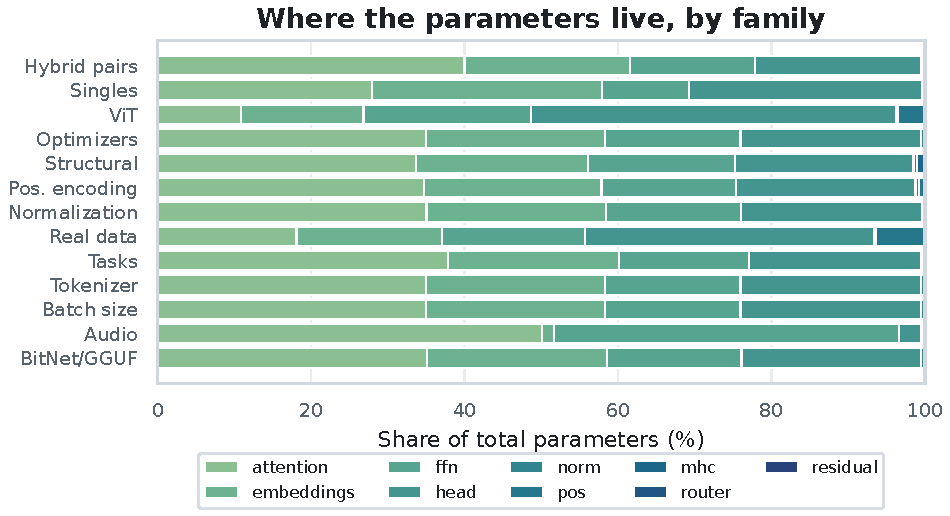
\includegraphics{../paper/figures/experiments/round2/params_composition.pdf}}
\caption{Dónde viven los parámetros, por familia. Los embeddings y la cabeza son costes fijos; el bloque de atención y la FFN cargan las diferencias arquitectónicas.}
\label{fig:r2-params-composition}
\end{figure}

\begin{figure}[tbp]
\centering
\fitfigure{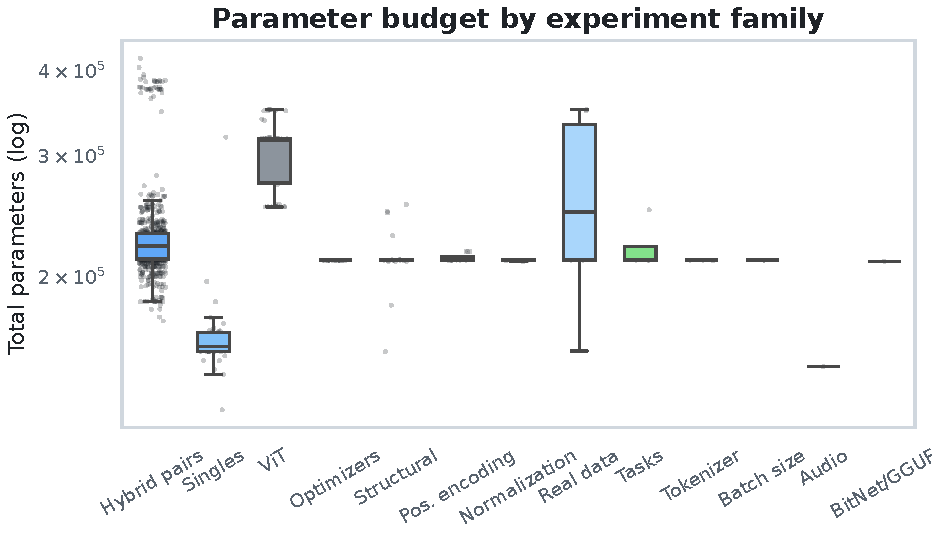
\includegraphics{../paper/figures/experiments/round2/params_family_box.pdf}}
\caption{Presupuesto de parámetros por familia de experimentos (escala log). La familia ViT es la más cara; las familias de ablación comparten un esqueleto.}
\label{fig:r2-params-family}
\end{figure}

\subsection{Resultados de entrenamiento}

Entre los pares híbridos, la pérdida final va de 8,116 a 10,450 nats (mediana 9,595). El mejor par es \texttt{nsa\_\_engram\_attn} con 8,116, seguido de \texttt{gated\_deltanet2\_\_sparda\_attn} (8,567) y \texttt{falcon3\_\_conformer\_attn} (8,620). El peor, \texttt{gqa\_\_tucker\_attn}, necesita 10,450 nats. La brecha entre extremos supera la brecha entre casi todas las ablaciones de optimizadores, y ese es el argumento más fuerte para elegir bien el par de atención.

Pérdida y precisión de validación no coinciden. Su correlación de rangos entre pares es débil, el par con mejor pérdida marca 0,0\% de top-1, y el de mejor precisión (\texttt{fox\_\_falcon1a\_attn}) alcanza 12,55\% con una pérdida de entrenamiento peor (9,292). Con cuatro frases de evaluación, un token afortunado reescribe el ranking, así que hay que reportar ambas señales. La Tabla~\ref{tab:r2-top-loss} lista los diez mejores pares por pérdida final y la Tabla~\ref{tab:r2-top-acc} los diez mejores por precisión de validación.

\begin{table}[H]
\centering
\small
\caption{Los diez mejores pares híbridos por pérdida final de entrenamiento.}
\label{tab:r2-top-loss}
\begin{tabular}{lrrrrr}
\toprule
Par (A + B) & Paráms. & Pérdida final & Top-1 & Top-5 & Entreno (min) \\
\midrule
\texttt{nsa + engram}              & 383\,999 & 8,116 & 0,00\% & 25,0\% & 154,5 \\
\texttt{gated\_deltanet2 + sparda} & 254\,336 & 8,567 & 0,00\% & 25,0\% & 78,2 \\
\texttt{falcon3 + conformer}       & 254\,640 & 8,620 & 4,67\% & 25,0\% & 32,6 \\
\texttt{falcon1a + conformer}      & 254\,640 & 8,633 & 2,38\% & 25,0\% & 23,0 \\
\texttt{falcon1 + conformer}       & 254\,640 & 8,639 & 4,67\% & 25,0\% & 21,3 \\
\texttt{fox + falcon2a}            & 222\,768 & 8,666 & 2,40\% & 25,0\% & 84,2 \\
\texttt{gqa + conformer}           & 242\,720 & 8,670 & 5,87\% & 25,0\% & 88,3 \\
\texttt{falcon3a + conformer}      & 254\,640 & 8,681 & 3,97\% & 25,0\% & 23,2 \\
\texttt{fox + falcon2}             & 222\,768 & 8,705 & 2,40\% & 25,0\% & 85,8 \\
\texttt{gla + engram}              & 387\,296 & 8,736 & 5,17\% & 25,0\% & 149,2 \\
\bottomrule
\end{tabular}
\end{table}

\begin{table}[H]
\centering
\small
\caption{Los diez mejores pares híbridos por precisión top-1 de validación.}
\label{tab:r2-top-acc}
\begin{tabular}{lrrrrr}
\toprule
Par (A + B) & Paráms. & Pérdida final & Top-1 & Top-5 & Entreno (min) \\
\midrule
\texttt{fox + falcon1a}             & 214\,232 & 9,292 & 12,55\% & 0,0\% & 79,3 \\
\texttt{fox + falcon3}              & 214\,232 & 9,618 & 12,55\% & 0,0\% & 106,1 \\
\texttt{fox + falcon3a}             & 214\,232 & 9,235 & 12,55\% & 0,0\% & 77,3 \\
\texttt{gated\_deltanet2 + falcon2} & 250\,216 & 9,105 & 12,41\% & 0,0\% & 80,7 \\
\texttt{gated\_deltanet2 + falcon2a} & 250\,216 & 8,968 & 12,41\% & 0,0\% & 82,1 \\
\texttt{hgrn2 + gated\_softmax}     & 238\,688 & 9,386 & 12,30\% & 25,0\% & 71,7 \\
\texttt{hgrn2 + tucker}             & 238\,688 & 9,221 & 12,30\% & 25,0\% & 81,6 \\
\texttt{gqla + mlra}                & 194\,624 & 9,461 & 11,85\% & 0,0\% & 56,0 \\
\texttt{mla + mlra}                 & 194\,624 & 9,464 & 11,85\% & 0,0\% & 86,6 \\
\texttt{deltanet + kda}             & 231\,304 & 9,024 & 11,37\% & 0,0\% & 78,6 \\
\bottomrule
\end{tabular}
\end{table}

\begin{figure}[tbp]
\centering
\fitfigure{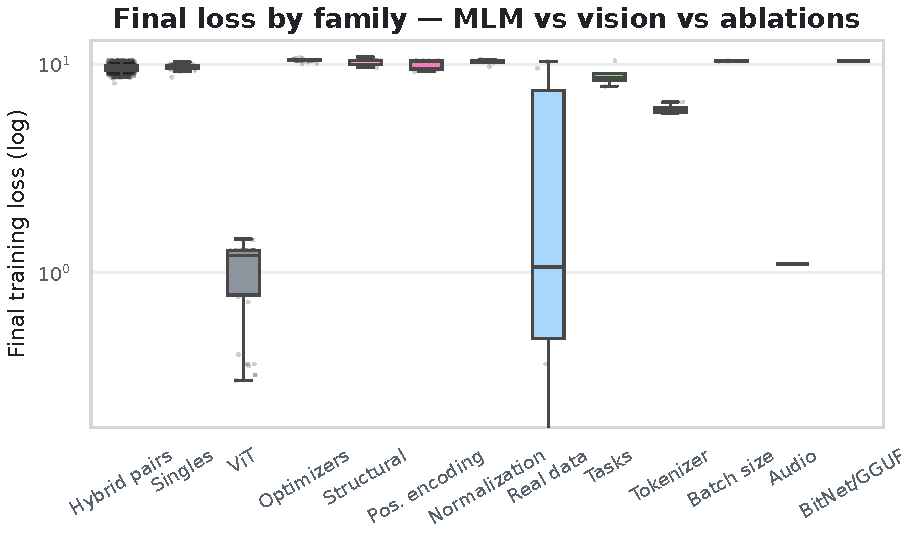
\includegraphics{../paper/figures/experiments/round2/loss_family_box.pdf}}
\caption{Pérdida final de entrenamiento por familia (escala log). Las familias de visión y datos reales no son comparables con las pérdidas MLM; las familias se mantienen separadas.}
\label{fig:r2-loss-family}
\end{figure}

\begin{figure}[tbp]
\centering
\fitfigure{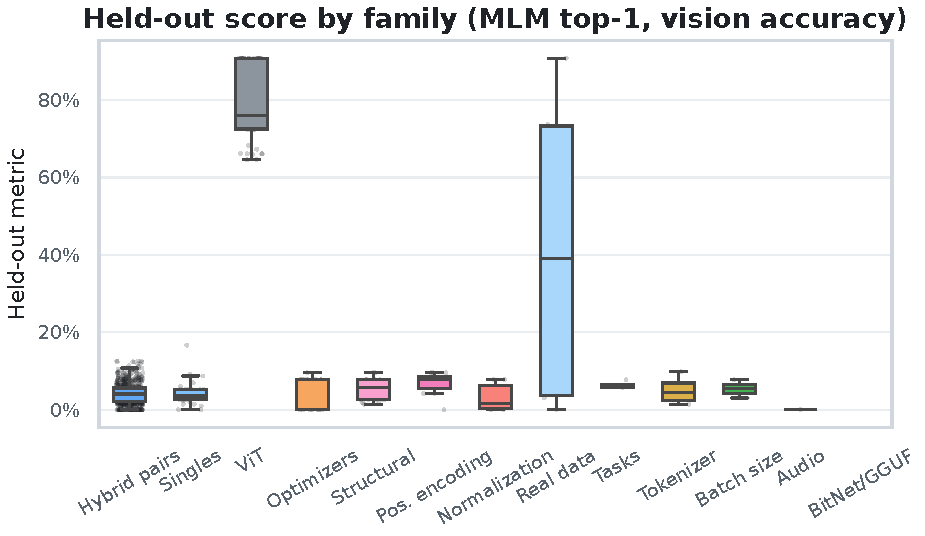
\includegraphics{../paper/figures/experiments/round2/acc_family_box.pdf}}
\caption{Métrica de validación por familia. Las tareas de visión puntúan un orden de magnitud por encima del MLM porque la tarea es más fácil, no porque el mezclador importe más.}
\label{fig:r2-acc-family}
\end{figure}

\begin{figure}[tbp]
\centering
\fitfigure{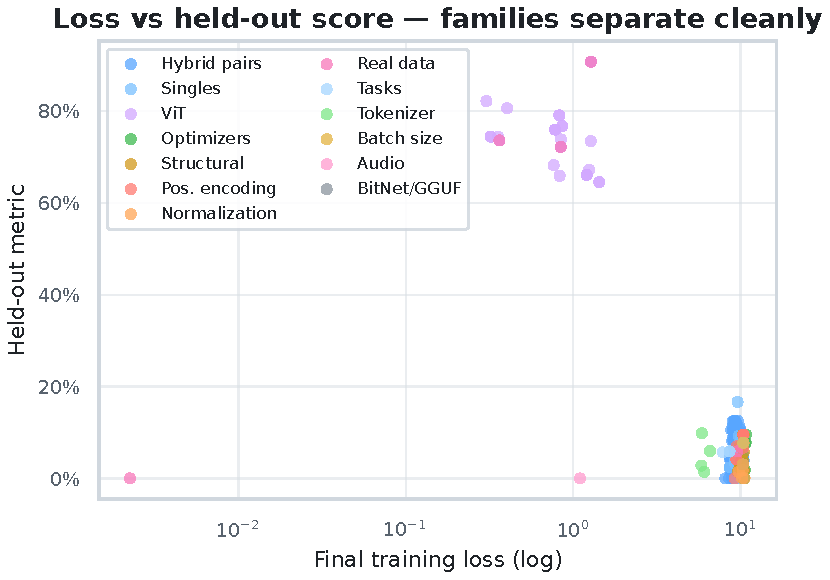
\includegraphics{../paper/figures/experiments/round2/loss_acc_scatter.pdf}}
\caption{Pérdida final frente a métrica de validación. La relación es débil dentro de los pares: el mejor par por pérdida marca 0,0\% de top-1 y el mejor por precisión tiene peor pérdida.}
\label{fig:r2-loss-acc}
\end{figure}

\subsection{Dinámica de entrenamiento}

Todas las corridas usan el mismo calendario de warm-up más coseno, así que las curvas de aprendizaje son directamente comparables. La población de pares sigue descendiendo en la época~100: la pérdida mediana cae de unos 10,2 nats en la época~0 a 9,49 al final. La tanda mide, por tanto, velocidad de aprendizaje y no calidad convergida, y todo ranking debe leerse como ``qué par aprende más rápido en 3{,}000 pasos''.

Las normas de gradiente son estables entre familias (1,87 para el bloque de atención, 0,92 para la FFN, 3,47 para la cabeza), y la razón de recorte mediana se sitúa en 0,90, por debajo del umbral de 1,0, así que la mayoría de los pasos pasan sin recorte y este solo actúa en los picos. El rendimiento mediano es 357 tokens/s para la población de pares; la cola de 3k--31k pertenece a ablaciones de tokenizer y audio cuyo cronómetro cubre solo parte del trabajo, por lo que el análisis de Pareto la excluye.

\begin{figure}[tbp]
\centering
\fitfigure{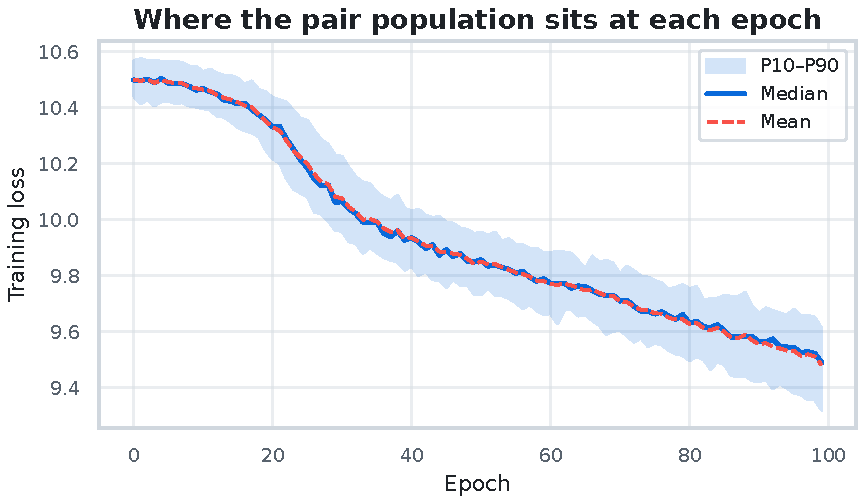
\includegraphics{../paper/figures/experiments/round2/curves_quantiles.pdf}}
\caption{Curvas de la población con banda P10--P90. Las curvas siguen bajando en la época~100, así que la tanda mide velocidad de aprendizaje y no calidad convergida.}
\label{fig:r2-curves-quantiles}
\end{figure}

\begin{figure}[tbp]
\centering
\fitfigure{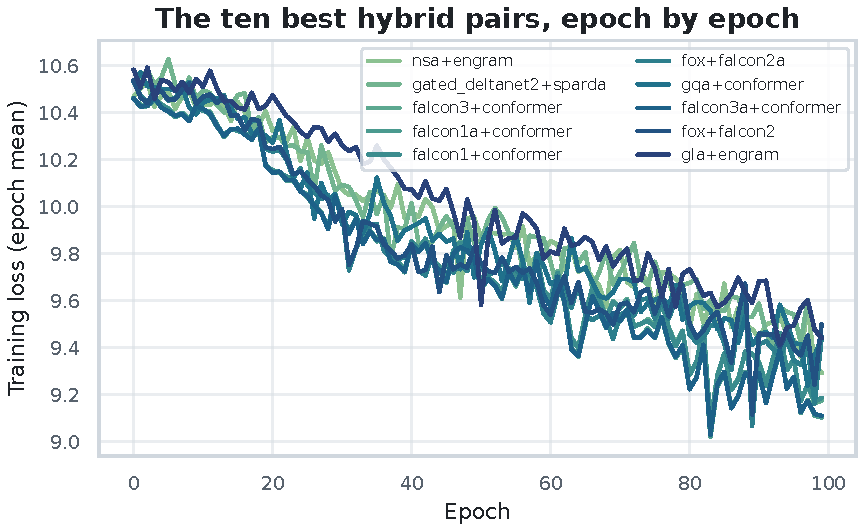
\includegraphics{../paper/figures/experiments/round2/curves_top10.pdf}}
\caption{Los diez mejores pares a lo largo del tiempo. El orden se establece pronto y rara vez cambia después de la época~50.}
\label{fig:r2-curves-top10}
\end{figure}

\begin{figure}[tbp]
\centering
\fitfigure{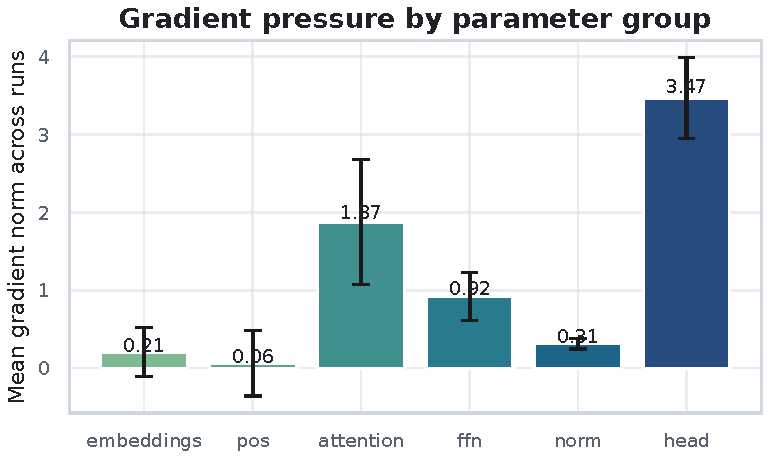
\includegraphics{../paper/figures/experiments/round2/grad_groups.pdf}}
\caption{Presión de gradiente por grupo de parámetros. La cabeza soporta el gradiente mayor y la FFN el menor; el recorte actúa rara vez porque la razón mediana es 0,90.}
\label{fig:r2-grad-groups}
\end{figure}

\subsection{El atlas A$\times$B}

El atlas es el centro del experimento: cada celda es un par híbrido, las filas son el primer mezclador y las columnas el segundo. Leído columna a columna, el segundo mezclador domina: un B bueno (\texttt{sparsek}, \texttt{engram}, \texttt{mlra}) mantiene casi todo A en la banda de 8,9--9,6 nats, mientras que un B malo (\texttt{mamba}, \texttt{retnet}, \texttt{bigbird}) arrastra incluso al mejor A por encima de 10 nats. Leído fila a fila, ningún primer mezclador rescata a un segundo malo.

La cobertura es casi completa: se entrenaron 667 de los 861 pares posibles. Los 158 pares que nunca entrenaron son exactamente los que contienen \texttt{cca}, \texttt{ccgqa}, \texttt{msa} o \texttt{ssog}, cuatro mezcladores que fallan en toda configuración ($4\times41 - \binom{4}{2} = 158$).

\begin{figure}[tbp]
\centering
\fitfigure{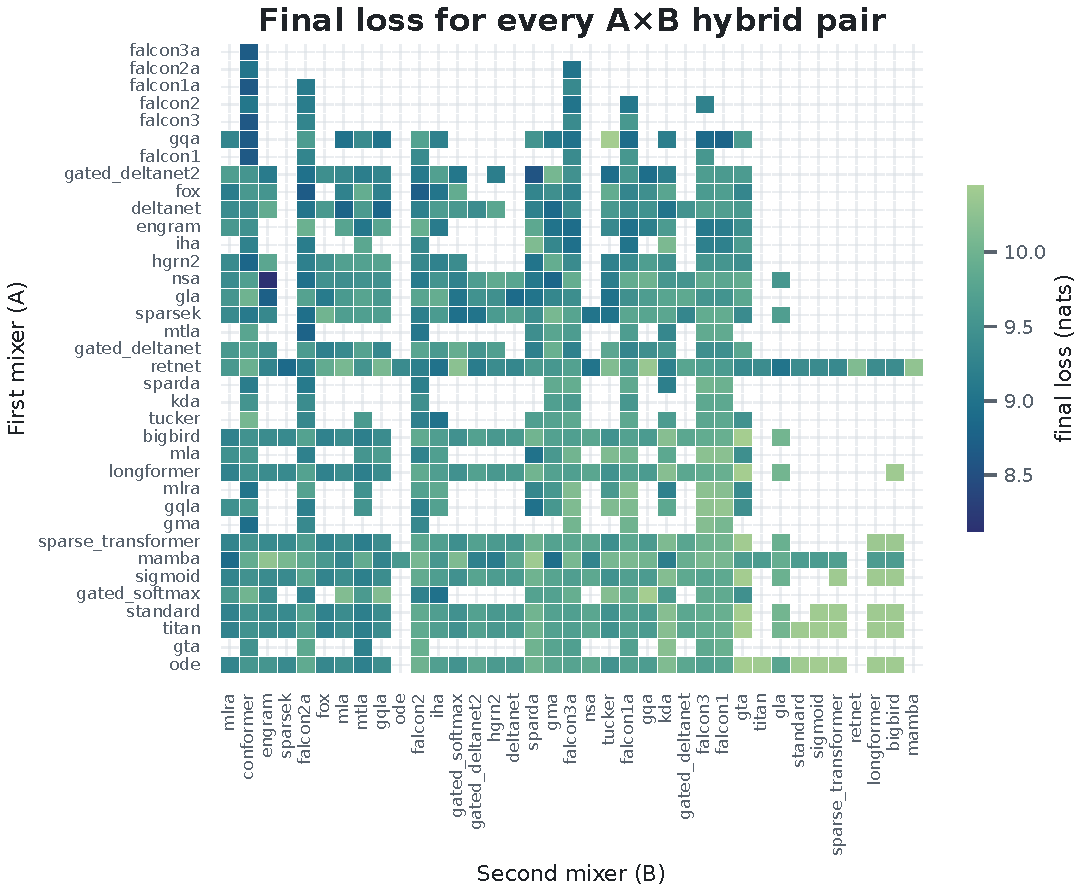
\includegraphics{../paper/figures/experiments/round2/matrix_loss.pdf}}
\caption{El atlas A$\times$B de pérdida final. Las filas son el primer mezclador y las columnas el segundo; las celdas vacías son pares que nunca entrenaron.}
\label{fig:r2-matrix-loss}
\end{figure}

\begin{figure}[tbp]
\centering
\fitfigure{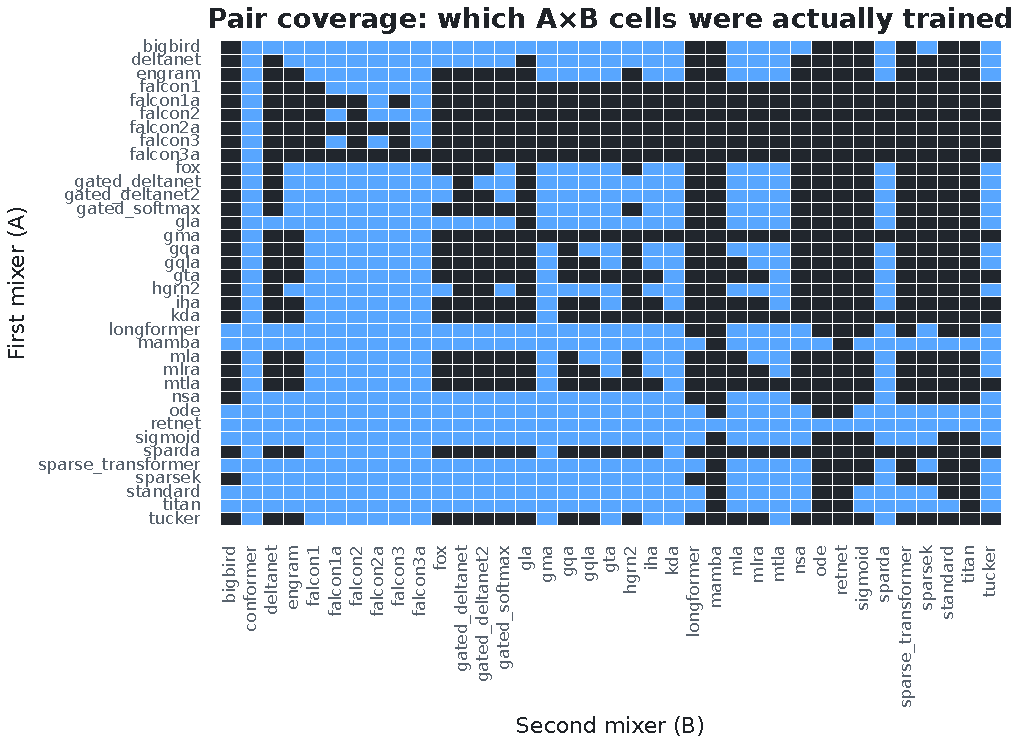
\includegraphics{../paper/figures/experiments/round2/coverage.pdf}}
\caption{Cobertura de la rejilla A$\times$B. Las celdas ausentes son los 158 pares que contienen uno de los cuatro mezcladores que nunca entrenan.}
\label{fig:r2-coverage}
\end{figure}

\paragraph{Qué segundo mezclador elegir.}
La Tabla~\ref{tab:r2-best-b} ordena los segundos mezcladores por pérdida final media en todos los pares que los contienen. La columna Pares indica el tamaño de muestra detrás de cada media; una media de un solo par (por ejemplo \texttt{mamba}) es anecdótica. La mitad inferior es tan informativa como la superior: \texttt{mamba}, \texttt{bigbird}, \texttt{longformer} y \texttt{retnet} son baratos pero arrastran sistemáticamente al par, justo el patrón que muestran los mapas de calor.

\begin{table}[H]
\centering
\small
\caption{Segundos mezcladores ordenados por pérdida final media en los pares que los contienen (mejores ocho y peores ocho).}
\label{tab:r2-best-b}
\begin{tabular}{lrrrr}
\toprule
Segundo mezclador & Pares & Pérdida media & Top-1 medio & Paráms. medios \\
\midrule
\texttt{mlra}        & 22 & 9,368 & 5,74\% & 209\,581 \\
\texttt{conformer}   & 36 & 9,369 & 3,39\% & 259\,861 \\
\texttt{engram}      & 18 & 9,373 & 2,05\% & 379\,284 \\
\texttt{sparsek}     & 9  & 9,382 & 4,82\% & 208\,926 \\
\texttt{falcon2a}    & 34 & 9,387 & 4,33\% & 229\,973 \\
\texttt{fox}         & 16 & 9,409 & 2,23\% & 216\,038 \\
\texttt{mla}         & 20 & 9,457 & 4,66\% & 217\,989 \\
\texttt{mtla}        & 26 & 9,459 & 5,29\% & 217\,223 \\
\midrule
\texttt{falcon1}     & 30 & 9,779 & 3,27\% & 221\,856 \\
\texttt{gta}         & 25 & 9,788 & 3,27\% & 219\,828 \\
\texttt{titan}       & 3  & 9,814 & 6,28\% & 204\,768 \\
\texttt{gla}         & 11 & 9,814 & 3,90\% & 222\,555 \\
\texttt{standard}    & 4  & 9,960 & 6,65\% & 206\,264 \\
\texttt{sigmoid}     & 5  & 10,045 & 4,37\% & 207\,162 \\
\texttt{sparse\_transformer} & 6 & 10,108 & 5,59\% & 207\,760 \\
\texttt{mamba}       & 1  & 10,279 & 2,04\% & 192\,608 \\
\bottomrule
\end{tabular}
\end{table}

\paragraph{La interacción supera a los marginales.}
El gráfico de sinergia mide cuánto mejor es un par frente a la media de sus dos marginales,
\[
S_{A,B} = \frac{\mu_A + \mu_B}{2} - L_{A,B},
\]
donde $\mu_A$ y $\mu_B$ son las pérdidas medias de todos los pares que contienen A y B. \texttt{nsa+engram} gana 1,304 nats y los diez primeros comparten un patrón: un primer mezclador barato y limpio con un segundo de memoria pesada. La cola negativa está dominada por \texttt{gta}, \texttt{gqa} y \texttt{tucker} como B---mezcladores que parecen promedio en aislamiento pero chocan al apilarse tras un A fuerte.

\begin{table}[H]
\centering
\small
\caption{Las mejores y peores interacciones entre mezcladores por sinergia. Los valores positivos indican que el par es mejor de lo que sugieren sus partes.}
\label{tab:r2-synergy}
\begin{tabular}{lrrrr}
\toprule
Par & Pérdida del par & Esperada & Sinergia & Top-1 \\
\midrule
\texttt{nsa + engram}              & 8,116  & 9,420 & $+1{,}304$ & 0,00\% \\
\texttt{gated\_deltanet2 + sparda} & 8,567  & 9,448 & $+0{,}881$ & 0,00\% \\
\texttt{fox + falcon2}             & 8,705  & 9,446 & $+0{,}741$ & 2,40\% \\
\texttt{gqa + falcon1}             & 8,784  & 9,518 & $+0{,}734$ & 2,86\% \\
\texttt{fox + falcon2a}            & 8,666  & 9,390 & $+0{,}724$ & 2,40\% \\
\midrule
\texttt{bigbird + gta}             & 10,445 & 9,725 & $-0{,}720$ & 1,79\% \\
\texttt{retnet + gated\_softmax}   & 10,239 & 9,533 & $-0{,}706$ & 7,70\% \\
\texttt{mamba + engram}            & 10,277 & 9,543 & $-0{,}734$ & 1,10\% \\
\texttt{mamba + sparda}            & 10,391 & 9,643 & $-0{,}749$ & 5,09\% \\
\texttt{gqa + tucker}              & 10,450 & 9,432 & $-1{,}018$ & 7,76\% \\
\bottomrule
\end{tabular}
\end{table}

\begin{figure}[tbp]
\centering
\fitfigure{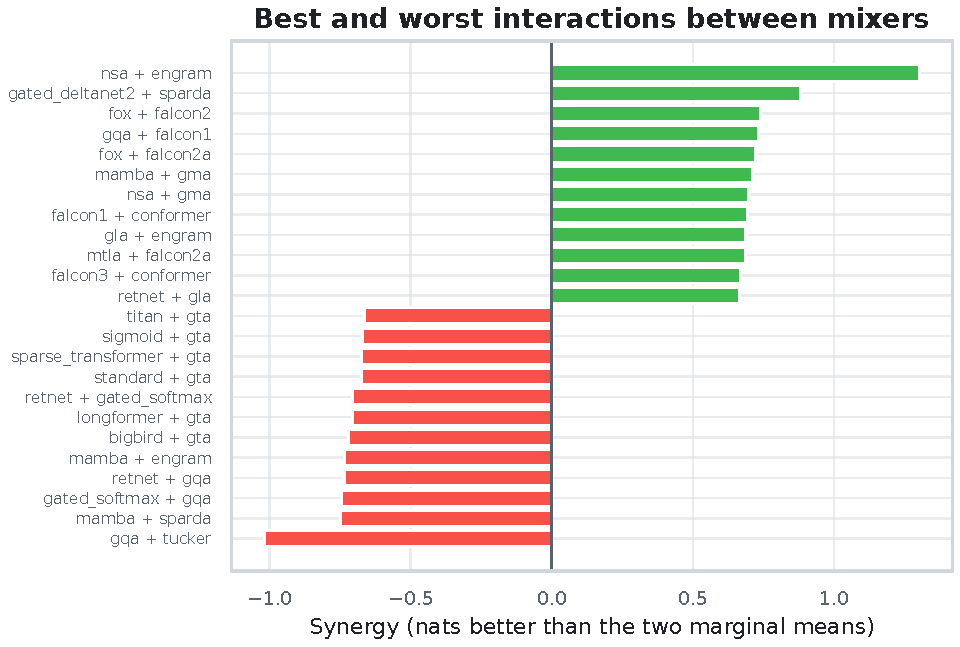
\includegraphics{../paper/figures/experiments/round2/synergy.pdf}}
\caption{Mejores y peores interacciones entre mixers. La cola positiva empareja un primer mezclador barato y estable con un segundo de memoria pesada; la cola negativa está dominada por segundos mezcladores que chocan tras un A fuerte.}
\label{fig:r2-synergy}
\end{figure}

\begin{figure}[tbp]
\centering
\fitfigure{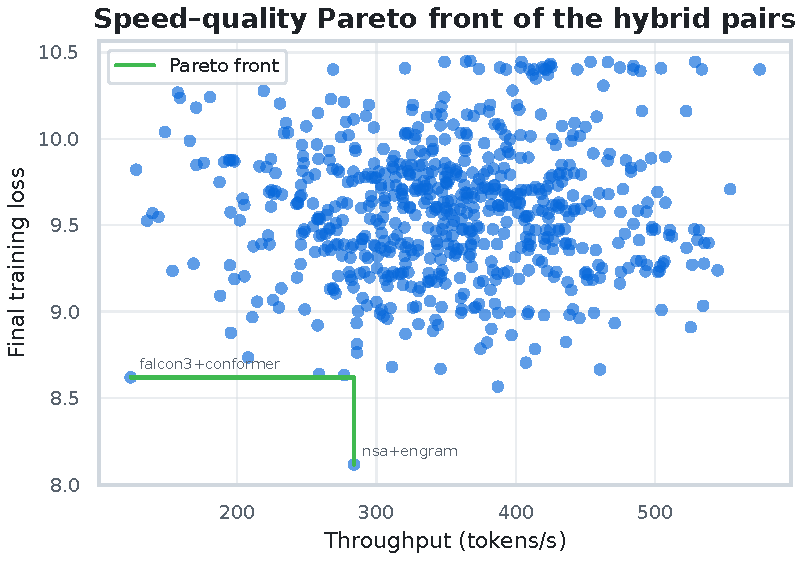
\includegraphics{../paper/figures/experiments/round2/pareto_speed_loss.pdf}}
\caption{Frontera de Pareto velocidad--calidad de los pares híbridos. La frontera la pueblan pares cuyo segundo mezclador tiene memoria pesada pero cuyo primero es barato.}
\label{fig:r2-pareto}
\end{figure}

\begin{figure}[tbp]
\centering
\fitfigure{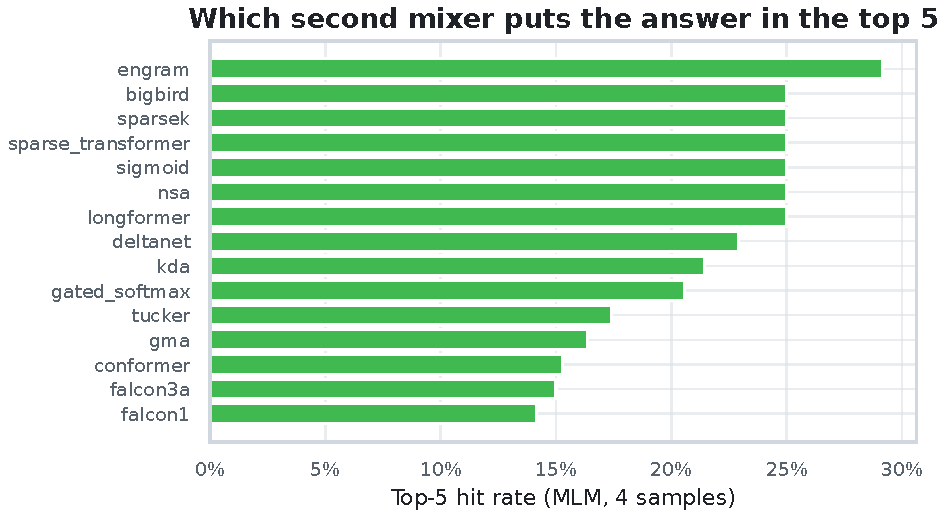
\includegraphics{../paper/figures/experiments/round2/top5_by_b.pdf}}
\caption{Top-5 por segundo mezclador. Con cuatro muestras por configuración, el intervalo entre barras adyacentes es una muestra, así que el orden es indicativo.}
\label{fig:r2-top5-b}
\end{figure}

\begin{figure}[tbp]
\centering
\fitfigure{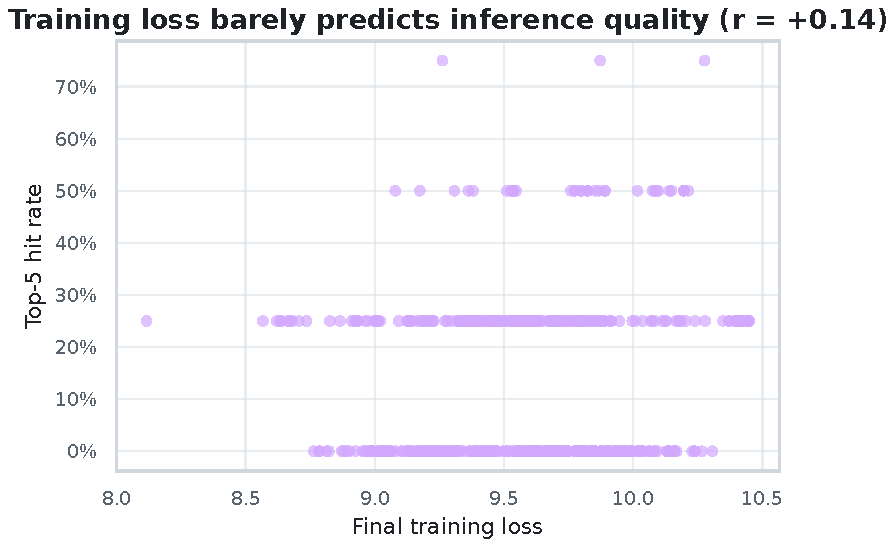
\includegraphics{../paper/figures/experiments/round2/top5_vs_loss.pdf}}
\caption{Calidad de inferencia frente a pérdida de entrenamiento. La correlación es débil ($r = 0{,}14$): la pérdida de entrenamiento no sustituye a la evaluación en validación.}
\label{fig:r2-top5-loss}
\end{figure}

\subsection{Ablaciones}

\paragraph{Optimizadores.}
La barrida de optimizadores es el gráfico más aleccionador: 23 optimizadores, el mismo esqueleto de 210k y un rango de 10,10--10,77 nats. \texttt{q\_apollo} gana con 10,098 y \texttt{galore\_adamw} cierra la tabla con 10,772, pero una docena de optimizadores aterrizan exactamente en 10,404, así que la corrida es demasiado corta para separar la elección del ruido de semilla. Las diferencias de velocidad sí son reales: el tiempo por paso varía un 30\% y \texttt{shampoo} y \texttt{muon} pagan sobrecoste visible.

\begin{table}[H]
\centering
\small
\caption{Ablación de optimizadores: pérdida final, top-1 de validación y rendimiento sobre el mismo esqueleto.}
\label{tab:r2-optimizers}
\begin{tabular}{lrrr}
\toprule
Optimizador & Pérdida final & Top-1 & Tok/s \\
\midrule
\texttt{q\_apollo}           & 10,098 & 3,63\% & 436 \\
\texttt{sophia}              & 10,104 & 1,79\% & 378 \\
\texttt{lion}                & 10,245 & 4,64\% & 279 \\
\texttt{shampoo}             & 10,401 & 7,76\% & 382 \\
\texttt{adopt}               & 10,404 & 7,76\% & 391 \\
\texttt{mars\_adamw}         & 10,404 & 7,76\% & 343 \\
\texttt{adan}                & 10,404 & 7,76\% & 359 \\
\texttt{adamw}               & 10,404 & 7,76\% & 384 \\
\texttt{schedulefree\_adamw} & 10,404 & 7,76\% & 487 \\
\texttt{soap}                & 10,404 & 7,76\% & 412 \\
\texttt{ademamix}            & 10,404 & 7,76\% & 366 \\
\texttt{cautious\_adamw}     & 10,404 & 7,76\% & 365 \\
\texttt{prodigy}             & 10,439 & 0,00\% & 349 \\
\texttt{sgd\_momentum}       & 10,450 & 0,00\% & 347 \\
\texttt{turbo\_muon}         & 10,454 & 0,00\% & 536 \\
\texttt{anon}                & 10,458 & 0,00\% & 387 \\
\texttt{muon}                & 10,461 & 0,00\% & 507 \\
\texttt{apollo}              & 10,519 & 0,00\% & 401 \\
\texttt{adafactor}           & 10,530 & 0,00\% & 395 \\
\texttt{ada\_muon}           & 10,620 & 1,79\% & 497 \\
\texttt{lamb}                & 10,653 & 7,76\% & 464 \\
\texttt{radam}               & 10,738 & 7,76\% & 502 \\
\texttt{galore\_adamw}       & 10,772 & 9,54\% & 451 \\
\bottomrule
\end{tabular}
\end{table}

\begin{figure}[tbp]
\centering
\fitfigure{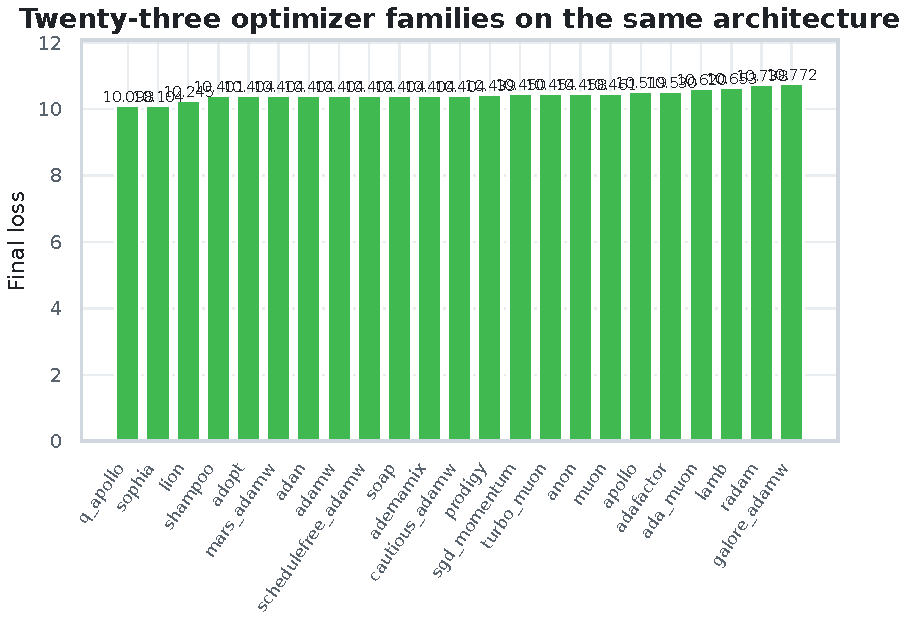
\includegraphics{../paper/figures/experiments/round2/opt_loss.pdf}}
\caption{Ablación de optimizadores: pérdida final. Una docena converge al mismo valor, lo que mide más la brevedad de la corrida que la calidad del optimizador.}
\label{fig:r2-opt-loss}
\end{figure}

\begin{figure}[tbp]
\centering
\fitfigure{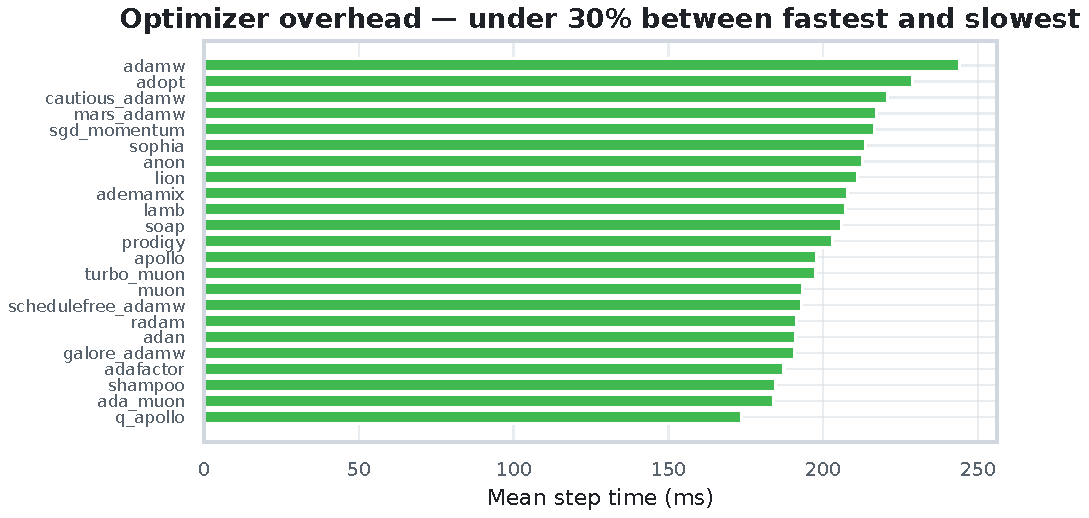
\includegraphics{../paper/figures/experiments/round2/opt_speed.pdf}}
\caption{Ablación de optimizadores: tiempo por paso medio. La dispersión es de un 30\%; los métodos de segundo orden y ortogonalizados pagan el sobrecoste visible.}
\label{fig:r2-opt-speed}
\end{figure}

\paragraph{Normalización y codificación posicional.}
Entre las normalizaciones, \texttt{flash\_norm} gana con claridad (9,749 nats, medio nat por delante del segundo), mientras que \texttt{prms\_norm} y \texttt{rms\_norm} quedan atrás. En codificaciones posicionales la familia PAPE (\texttt{pape\_ri}, \texttt{pape}, \texttt{pape\_efficient}) barre el podio, y RoPE clásico queda a media tabla a esta escala---recordatorio de que ``moderno'' no es automáticamente mejor en una corrida de 100 épocas.

\begin{table}[H]
\centering
\small
\caption{Ablación de normalización sobre el esqueleto compartido.}
\label{tab:r2-norms}
\begin{tabular}{lrrr}
\toprule
Variante & Pérdida final & Top-1 & Paráms. \\
\midrule
\texttt{flash\_norm}   & 9,749  & 1,43\% & 209\,600 \\
\texttt{dynamic\_tanh} & 10,246 & 0,00\% & 210\,752 \\
\texttt{derf}          & 10,295 & 1,79\% & 210\,762 \\
\texttt{layer\_norm}   & 10,401 & 7,76\% & 210\,752 \\
\texttt{rms\_norm}     & 10,436 & 7,76\% & 210\,272 \\
\texttt{prms\_norm}    & 10,573 & 0,00\% & 210\,272 \\
\bottomrule
\end{tabular}
\end{table}

\begin{table}[H]
\centering
\small
\caption{Ablación de codificación posicional.}
\label{tab:r2-pe}
\begin{tabular}{lrrr}
\toprule
Codificación & Pérdida final & Top-1 & Paráms. \\
\midrule
\texttt{pari}                 & 9,235  & 0,00\% & 211\,520 \\
\texttt{pape}                 & 9,455  & 4,17\% & 216\,928 \\
\texttt{pape\_efficient}      & 9,455  & 4,17\% & 216\,928 \\
\texttt{learned\_absolute}    & 9,525  & 7,02\% & 216\,896 \\
\texttt{hope}                 & 10,348 & ---    & 210\,752 \\
\texttt{sinusoidal\_absolute} & 10,364 & 6,68\% & 210\,752 \\
\texttt{bam}                  & 10,397 & 9,54\% & 210\,768 \\
\texttt{nope}                 & 10,397 & 9,54\% & 210\,752 \\
\texttt{none}                 & 10,397 & 9,54\% & 210\,752 \\
\texttt{rope}                 & 10,401 & 7,76\% & 210\,752 \\
\texttt{sinusoidal\_rotary}   & 10,401 & 7,76\% & 210\,752 \\
\texttt{alibi}                & 10,417 & 7,76\% & 210\,752 \\
\bottomrule
\end{tabular}
\end{table}

\begin{figure}[tbp]
\centering
\fitfigure{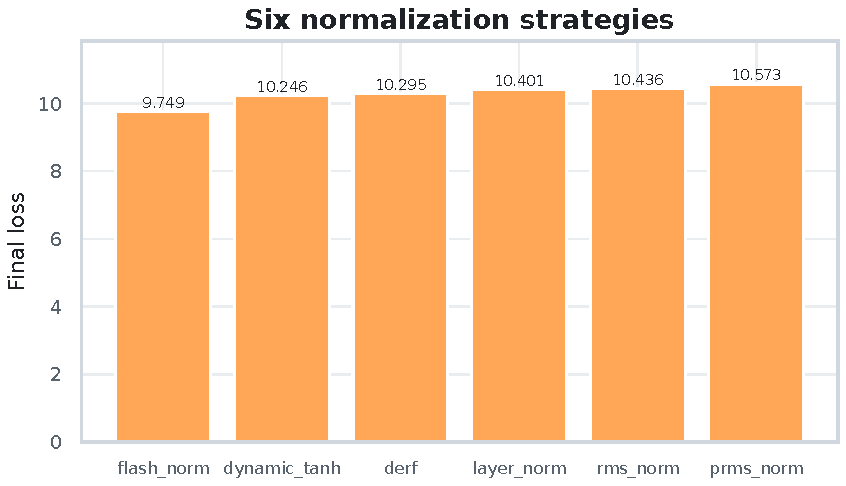
\includegraphics{../paper/figures/experiments/round2/norm_loss.pdf}}
\caption{Ablación de normalización: \texttt{flash\_norm} se separa del resto por medio nat.}
\label{fig:r2-norm}
\end{figure}

\begin{figure}[tbp]
\centering
\fitfigure{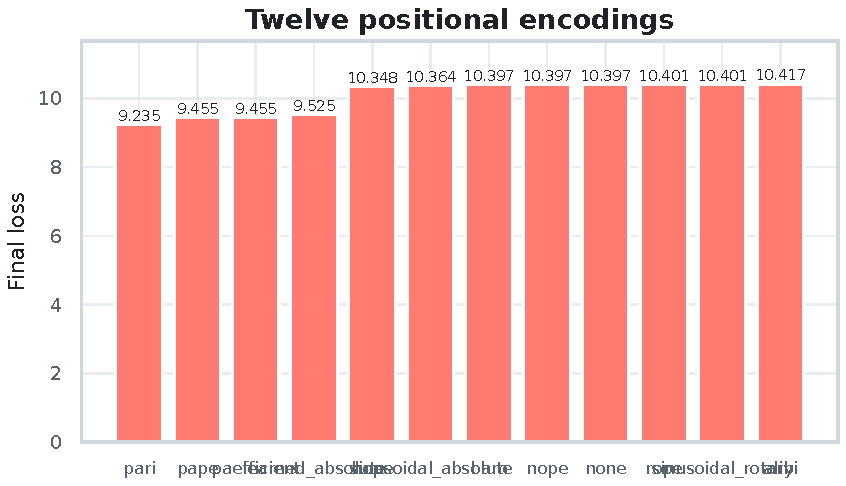
\includegraphics{../paper/figures/experiments/round2/pe_loss.pdf}}
\caption{Ablación de codificación posicional: la familia PAPE lidera y RoPE clásico queda a media tabla a esta escala.}
\label{fig:r2-pe}
\end{figure}

\paragraph{Conmutadores estructurales.}
Los conmutadores estructurales se separan más que los optimizadores. Los embeddings factorizados (9,623), la FFN SwiGLU (9,901) y dos bucles de Hyperloop (9,908) son las tres victorias; los conmutadores de BitNet quedan en 10,016, mHC en 10,186 y las variantes de residuales en 10,43--10,49. Mixture-of-Depths es el peor conmutador con 10,854, consistente con su incompatibilidad con mHC a esta profundidad.

\begin{table}[H]
\centering
\small
\caption{Conmutadores estructurales, ordenados por pérdida final.}
\label{tab:r2-trans}
\begin{tabular}{lrrr}
\toprule
Conmutador & Pérdida final & Top-1 & Paráms. \\
\midrule
\texttt{factorized\_emb}              & 9,623  & 1,43\% & 181\,056 \\
\texttt{ffn\_swiglu}                  & 9,901  & 2,49\% & 228\,800 \\
\texttt{num\_loops\_2}                & 9,908  & 6,94\% & 154\,880 \\
\texttt{fixed\_softmax\_ssmax\_bitnet} & 9,936 & 2,60\% & 209\,864 \\
\texttt{bitnet\_conv}                 & 10,016 & 2,60\% & 209\,856 \\
\texttt{bitnet\_on}                   & 10,016 & 2,60\% & 209\,856 \\
\texttt{mhc}                          & 10,186 & 1,79\% & 254\,092 \\
\texttt{bitnet\_routers}              & 10,327 & ---    & 247\,104 \\
\texttt{ssmax}                        & 10,359 & 9,54\% & 210\,760 \\
\texttt{ffn\_relu}                    & 10,393 & 3,83\% & 210\,752 \\
\texttt{fixed\_both}                  & 10,401 & 7,76\% & 210\,752 \\
\texttt{embedding\_conv}              & 10,401 & 7,76\% & 210\,752 \\
\texttt{fixed\_ce}                    & 10,401 & 7,76\% & 210\,752 \\
\texttt{pos\_rope}                    & 10,401 & 7,76\% & 210\,752 \\
\texttt{fixed\_softmax}               & 10,401 & 7,76\% & 210\,752 \\
\texttt{residuals\_full\_attn}        & 10,433 & 9,54\% & 210\,944 \\
\texttt{residuals\_none}              & 10,476 & 5,71\% & 210\,752 \\
\texttt{moe}                          & 10,477 & ---    & 248\,384 \\
\texttt{residuals\_block\_attn}       & 10,487 & 1,79\% & 210\,944 \\
\texttt{mod}                          & 10,854 & --- & 210\,944 \\
\bottomrule
\end{tabular}
\end{table}

\begin{figure}[tbp]
\centering
\fitfigure{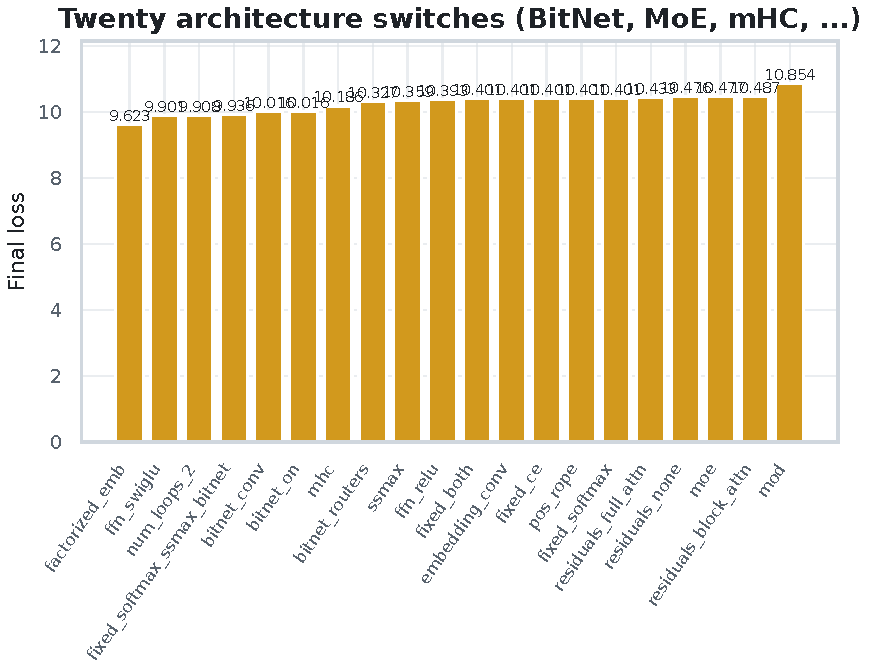
\includegraphics{../paper/figures/experiments/round2/trans_loss.pdf}}
\caption{Conmutadores estructurales. Los embeddings factorizados, SwiGLU y Hyperloop son las tres victorias; Mixture-of-Depths es el peor conmutador.}
\label{fig:r2-trans}
\end{figure}

\paragraph{Visión y tareas.}
El bloque de visión funciona. La segmentación alcanza 90,7\% de precisión media de validación, la clasificación 75,8\% y la predicción de parches 69,9\%. Estas cifras están un orden de magnitud por encima de los pares MLM (mediana 4,0\%) porque la tarea es más fácil, no porque el mezclador importe más, y por eso el informe mantiene las familias separadas. Las ablaciones de tokenizer y tarea se comportan como se espera: el tokenizer cambia la pérdida en varios nats porque cambia el vocabulario y la longitud media de secuencia, y la tarea la cambia porque cambia el objetivo.

\begin{figure}[tbp]
\centering
\fitfigure{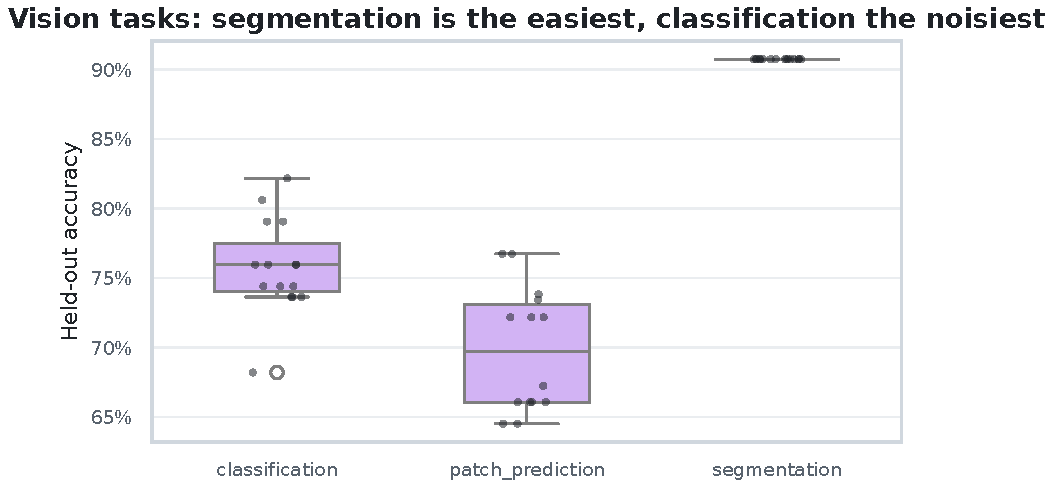
\includegraphics{../paper/figures/experiments/round2/vit_split.pdf}}
\caption{Tareas de visión por objetivo. La segmentación es la más fácil y la predicción de parches la más difícil.}
\label{fig:r2-vit}
\end{figure}

\begin{figure}[tbp]
\centering
\fitfigure{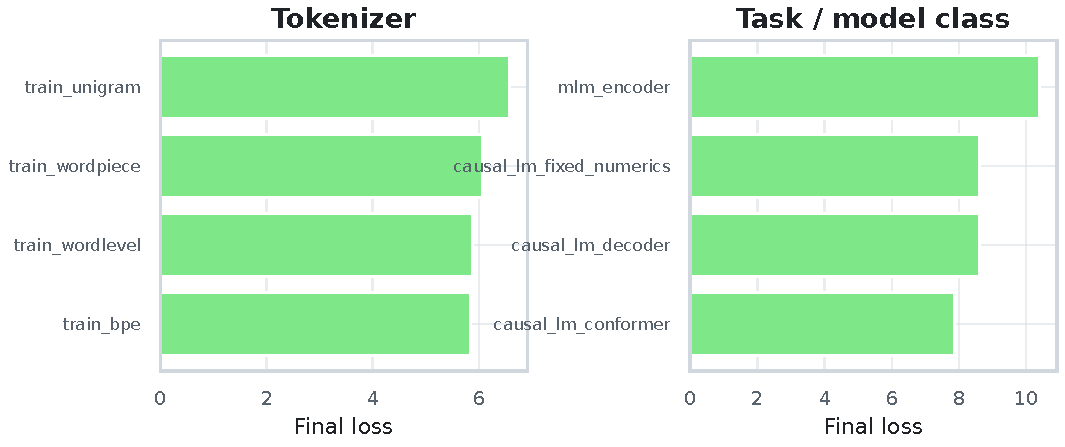
\includegraphics{../paper/figures/experiments/round2/tokenizer_task.pdf}}
\caption{Ablaciones de tokenizer y tarea. Ambas cambian la escala de la pérdida, así que no son comparables con la barrida de mezcladores.}
\label{fig:r2-tokenizer-task}
\end{figure}

\subsection{Despliegue e inferencia}

La cuantización post-entrenamiento es la buena noticia de la ronda. En las 810 configuraciones con ambos formatos, el top-1 medio pasa de 5,62\% a 5,43\% y el top-5 medio de 13,36\% a 13,24\%, deltas de $-0{,}19$ y $-0{,}12$ puntos porcentuales. Ochocientas configuraciones quedan exactamente iguales; las pocas que se mueven lo hacen por una muestra de cuatro. Para un modelo a escala de humo es el resultado esperado, pero vale la pena medirlo en vez de asumirlo.

La historia de velocidad es menos halagüeña. El despliegue cuantizado es más rápido que el estándar solo en el 32,3\% de las corridas (ratio mediano 0,64$\times$) porque la etapa de despliegue está dominada por la serialización y la conversión, no por la inferencia; la evaluación es más rápida el 51,2\% de las veces con una aceleración mediana de 1,03$\times$. La inferencia en sí tarda unos 10,5\,s para cuatro frases, que es la métrica que importa en producción.

La mejor configuración de inferencia no es la de mejor pérdida. \texttt{mamba\_\_engram\_attn} acierta tres de cuatro tokens en el top-5 (75,0\%) con una pérdida de entrenamiento de 10,277, por encima de la mediana de los pares. Con cuatro muestras por configuración, el top-5 es un instrumento romo: sirve para detectar fallos catastróficos, no para coronar un ganador.

\begin{figure}[tbp]
\centering
\fitfigure{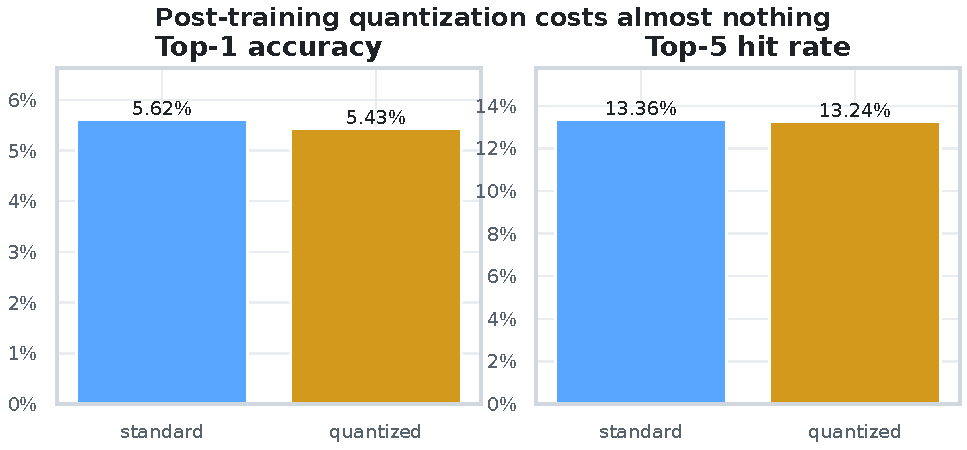
\includegraphics{../paper/figures/experiments/round2/inference_format.pdf}}
\caption{Inferencia estándar frente a cuantizada. Las distribuciones se solapan casi por completo.}
\label{fig:r2-inference-format}
\end{figure}

\begin{figure}[tbp]
\centering
\fitfigure{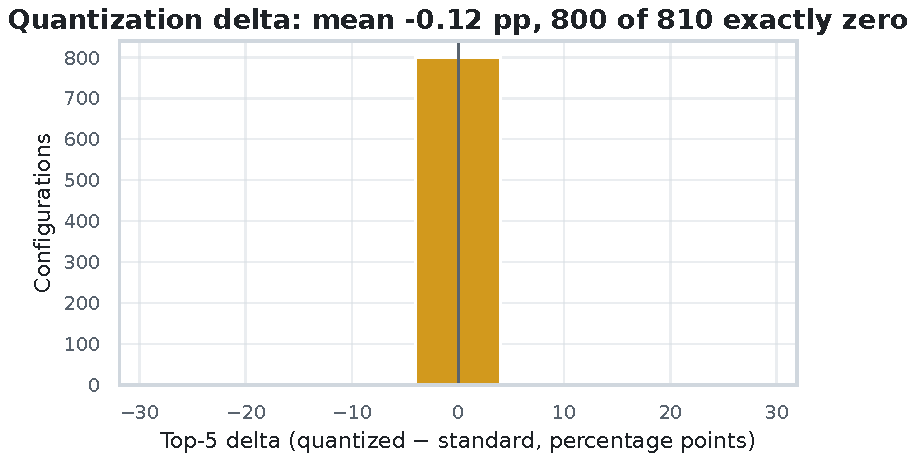
\includegraphics{../paper/figures/experiments/round2/quant_delta_dist.pdf}}
\caption{Distribución del delta de cuantización. Ochocientas de 810 configuraciones tienen un delta exactamente cero.}
\label{fig:r2-quant-delta}
\end{figure}

\begin{figure}[tbp]
\centering
\fitfigure{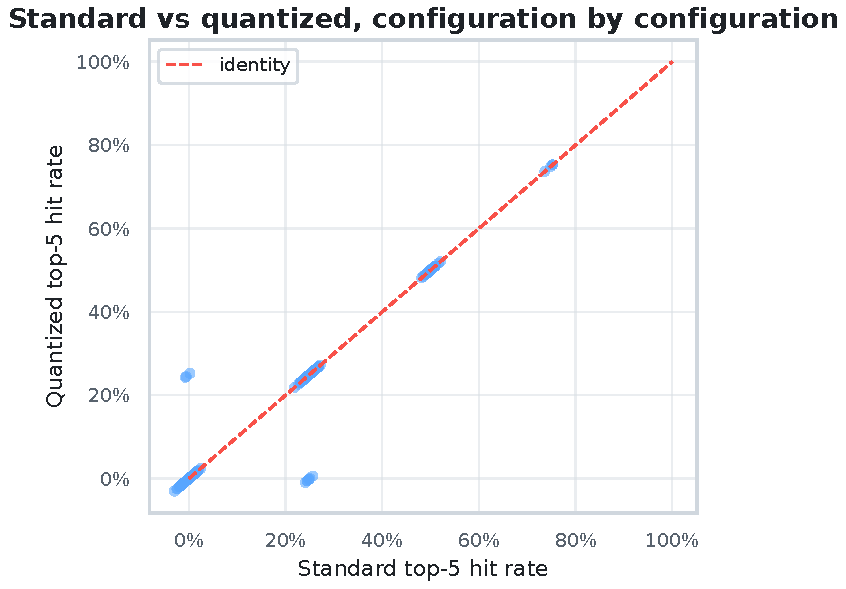
\includegraphics{../paper/figures/experiments/round2/quant_scatter.pdf}}
\caption{Top-5 estándar frente a cuantizado. Cada punto en la diagonal es una configuración que la cuantización no cambió.}
\label{fig:r2-quant-scatter}
\end{figure}

\begin{figure}[tbp]
\centering
\fitfigure{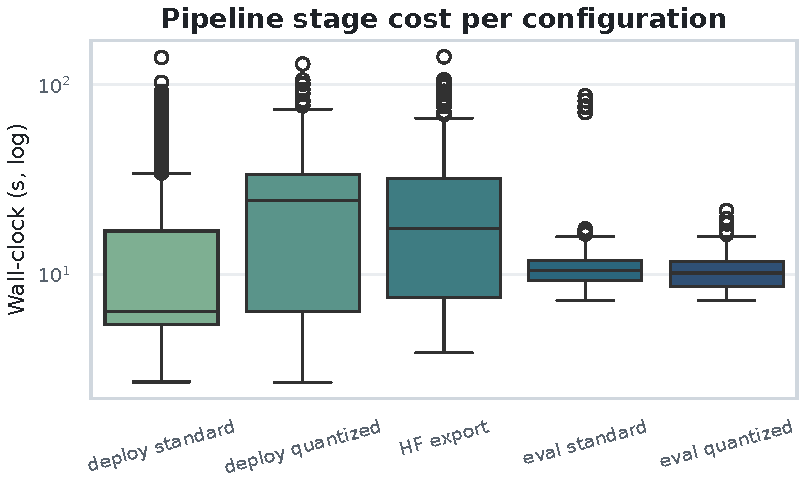
\includegraphics{../paper/figures/experiments/round2/deploy_duration.pdf}}
\caption{Coste por etapa del pipeline. El despliegue y la evaluación cuestan segundos; el entrenamiento cuesta horas.}
\label{fig:r2-deploy-duration}
\end{figure}

\begin{table}[H]
\centering
\small
\caption{Configuraciones con mejor tasa top-5 en formato estándar.}
\label{tab:r2-inference}
\begin{tabular}{lrrrrr}
\toprule
Configuración & Top-5 est. & Top-1 est. & Top-5 cuant. & Pérdida final & Paráms. \\
\midrule
\texttt{mamba\_\_engram\_attn} & 75\% & 50\% & 75\% & 10,277 & 347\,168 \\
\texttt{mamba\_\_nsa\_attn}    & 75\% & 0\%  & 75\% & 9,262  & 192\,479 \\
\texttt{retnet\_\_fox\_attn}  & 75\% & 0\%  & 75\% & 9,873  & 220\,936 \\
\texttt{bigbird\_\_kda\_attn}  & 50\% & 0\%  & 50\% & 10,196 & 221\,128 \\
\texttt{fox\_\_engram\_attn}   & 50\% & 25\% & 50\% & 9,535  & 375\,496 \\
\texttt{fox\_\_gated\_softmax\_attn} & 50\% & 25\% & 50\% & 9,892 & 220\,744 \\
\texttt{fox\_\_tucker\_attn}   & 50\% & 25\% & 50\% & 9,890  & 220\,744 \\
\texttt{gated\_deltanet\_\_tucker\_attn} & 50\% & 25\% & 50\% & 9,796 & 230\,928 \\
\texttt{gla\_\_falcon1\_attn}  & 50\% & 0\%  & 50\% & 9,511  & 226\,032 \\
\texttt{gla\_\_mlra\_attn}     & 50\% & 25\% & 50\% & 9,538  & 211\,808 \\
\bottomrule
\end{tabular}
\end{table}

\subsection{Fiabilidad del pipeline}

El libro registra 5{,}271 ejecuciones de etapas. 868 entrenamientos tuvieron éxito y 171 fallaron con código de salida distinto de cero, todos fuera de las 868 configuraciones analizadas, que se eligieron justamente porque entrenaron. El despliegue falló 104 veces de 1{,}734, siempre en pares simétricos: una configuración que falla el export estándar también falla el cuantizado, lo que apunta a una causa raíz compartida (serialización del checkpoint o de la configuración) y no a la cuantización en sí.

Dos hallazgos de calidad de datos condicionan la interpretación. Primero, cuatro mixers nunca entrenan: \texttt{cca}, \texttt{ccgqa}, \texttt{msa} y \texttt{ssog} fallan en sus cuatro singles y en los 158 pares que los contienen, exactamente las 158 celdas ausentes del atlas. Segundo, cuatro mixers son indistinguibles con contexto de 32 tokens: \texttt{standard}, \texttt{bigbird}, \texttt{longformer} y \texttt{titan} comparten pérdidas y parámetros bit a bit idénticos porque sus ventanas (al menos 64 tokens) cubren toda la secuencia y la variante aumentada con posición se reduce a atención multi-cabeza pura; coinciden en los 33 segundos mixers compartidos. Por separado, 37 pares aparecen como \texttt{attn\_retnet\_\_X} y \texttt{attn\_retnet\_attn\_\_X} con métricas idénticas---dos nombres para una implementación---que el atlas colapsa a una fila.

\begin{figure}[tbp]
\centering
\fitfigure{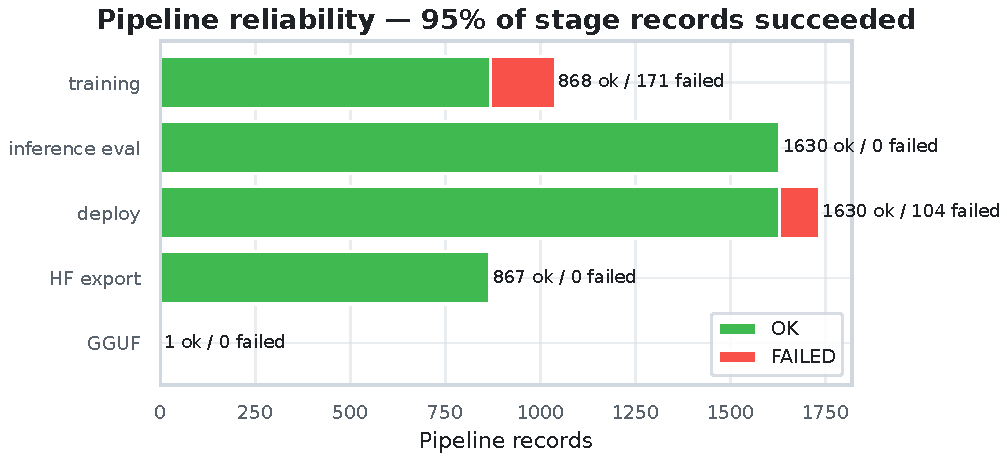
\includegraphics{../paper/figures/experiments/round2/stage_status.pdf}}
\caption{Fiabilidad del pipeline. El 95\% de los registros de etapa tuvo éxito; entrenamiento y despliegue explican todos los fallos.}
\label{fig:r2-stage-status}
\end{figure}

\begin{figure}[tbp]
\centering
\fitfigure{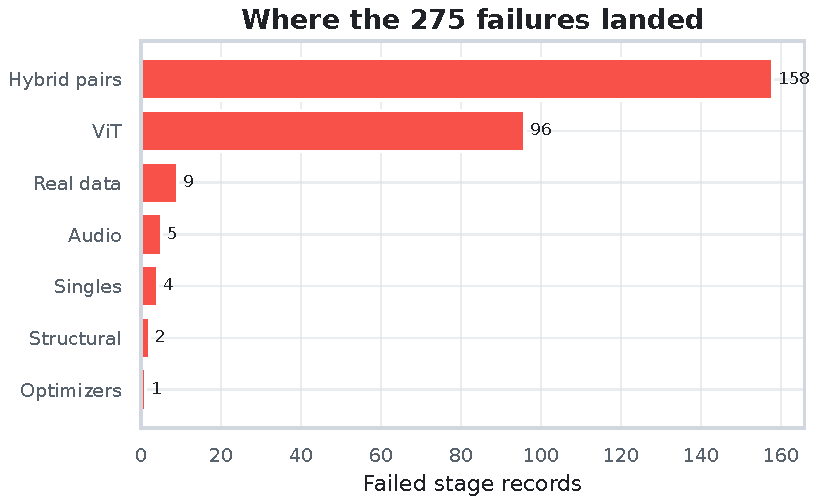
\includegraphics{../paper/figures/experiments/round2/failures_family.pdf}}
\caption{Dónde cayeron los 275 fallos. Los fallos de entrenamiento se concentran en las familias cuyos mezcladores nunca entrenan; los de despliegue son simétricos entre formatos.}
\label{fig:r2-failures}
\end{figure}

\subsection{Qué predice la calidad}

Sobre los pares híbridos, el número de parámetros correlaciona con la pérdida final a $r = -0{,}20$ y con la precisión de validación a $r = -0{,}07$: el tamaño apenas compra calidad aquí. Lo que sí predice de forma fiable es el coste ($r = 0{,}68$ con el tiempo por paso, $r = 0{,}65$ con el tiempo total). La pérdida de entrenamiento apenas informa sobre la calidad de inferencia ($r = 0{,}14$ con el top-5). La norma de gradiente y la razón de recorte son exactamente redundantes entre sí ($r = 1{,}00$), lo que es esperable porque la razón de recorte se calcula a partir de la norma de gradiente, y ninguna correlaciona con la calidad.

La matriz de correlación de la Figura~\ref{fig:r2-correlation} se calcula sobre las 868 filas. Leída así, el número de parámetros correlaciona con la pérdida a $-0{,}43$ y con la precisión a $+0{,}42$, lo que contradice los números de solo pares. Ambas lecturas son correctas: la matriz de todas las filas está dominada por el contraste entre transformers de visión (más grandes, mucha menor pérdida, mucha mayor precisión) y pares MLM, así que mide la brecha de familias y no el efecto del tamaño. Dentro de la población que importa para el atlas---los pares híbridos---el tamaño es casi irrelevante.

\begin{figure}[tbp]
\centering
\fitfigure{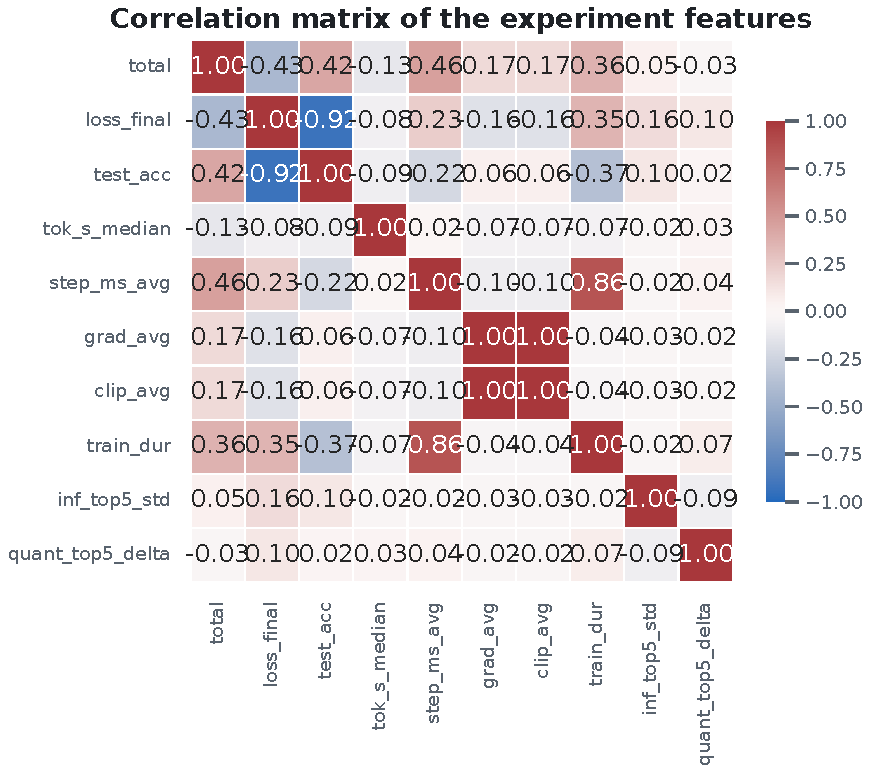
\includegraphics{../paper/figures/experiments/round2/correlation.pdf}}
\caption{Matriz de correlación sobre las 868 configuraciones. Las fuertes correlaciones parámetros--calidad son una confusión de familias; dentro de los pares híbridos caen a $-0{,}20$ y $-0{,}07$.}
\label{fig:r2-correlation}
\end{figure}

\subsection{Lectura práctica y próximos pasos}

Si hay que elegir a ciegas, usa un segundo mezclador con memoria pesada (\texttt{engram}, \texttt{sparsek}, \texttt{mlra}) y un primero barato y estable (\texttt{fox}, \texttt{gqa}, \texttt{gated\_deltanet2}), y evita \texttt{mamba}, \texttt{retnet} y \texttt{bigbird} como B. Espera unos $\pm0{,}3$ nats de ruido de interacción, mayor que la diferencia entre la mayoría de los optimizadores.

La ronda también define a su propia sucesora. El atlas debería repetirse con 256--512 tokens, donde los cuatro mezcladores que colapsan se vuelven distinguibles y los patrones dispersos se dispersan de verdad; la evaluación debería usar un conjunto reservado de 200 frases con log-verosimilitud por token, porque cuatro frases no pueden ordenar 800 configuraciones; los mejores pares deberían entrenarse 300 épocas, porque todas las curvas siguen bajando; el alias \texttt{retnet} y los cuatro mezcladores que fallan deberían corregirse o retirarse de la lista; y deberían correrse al menos tres semillas en las familias de ablación, donde la dispersión actual está dentro del ruido de semilla. La cuantización debería ser el formato de despliegue por defecto: costó 0,12 puntos de top-5 y aceleró la evaluación en la mitad de las corridas.
